\chapter{Discrete Hopfield Networks}
\label{ch:DHopfield}

In this chapter we are going to resume the notes of the course of Mathematical Models for Neural Networks of \citet{MMNN}. In particular, we are going to talk about the derivation of Hopfield neural networks and their properties. We are going to start from the derivation as a neural network with discrete states and finally we are going to use the perspective of statistical mechanics to analyze these neural networks.

\section{Derivation}

It's possible to make a mathematical model in order to analyze a natural neural network. Each neuron is a node of a graph and each synapse is an edge. A neural network is thus a graph.

\noindent Let two neurons, $A$ and $B$, be linked by a synapse. With respect to neuron $A$, we say that $A$ is a post-synaptic neuron and $B$ is a pre-synaptic neuron. A post-synaptic neuron receives information from all possible pre-synaptic neurons. This information consists of positive or negative ions, or even hormones that stimulate or alter the behavior of the neuron. In particular, these neurotransmitters either increase or decrease the potential of the neuron. If this potential exceeds a threshold, the neuron sends a message to the post-synaptic neurons and resets the potential. In \cref{fig:simple_diagram}, we show a simple diagram of the interaction between pre-synaptic and post-synaptic neurons.
\begin{figure}[htbp]
    \centering
    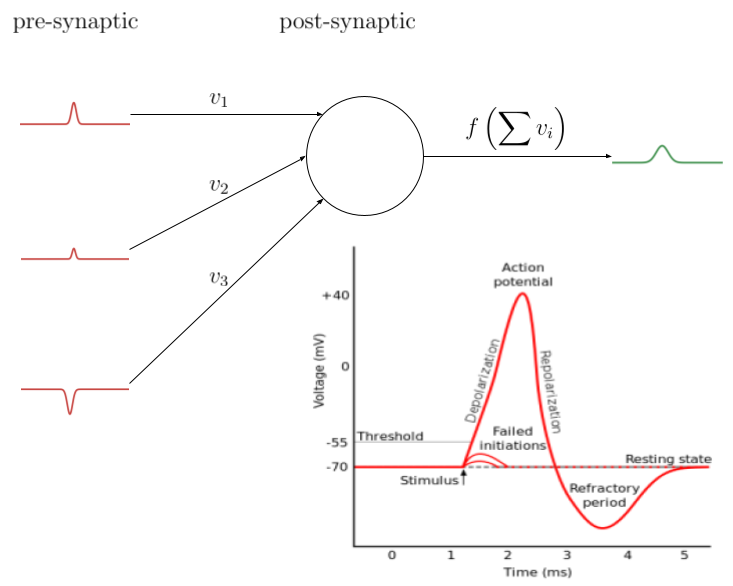
\includegraphics[width=0.8\linewidth]{Figures/simple_diagram.png}
    \caption{Pre-synaptic neurons send a signal to the post-synaptic neuron as a change in potential. The post-synaptic neuron accumulates all signals and generates a new signal if its potential exceeds a threshold.}
    \label{fig:simple_diagram}
\end{figure}
\begin{notation} In this article we denote with:
    \begin{itemize}
        \item[$U_i^t$] The potential of ${i}^\mathrm{th}$ neuron at time $t$.
        \item[$S_i^t$] The signal of ${i}^\mathrm{th}$ neuron at time $t$ from post-synaptic neurons.
        \item[$U_i^\star$] the threshold of ${i}^\mathrm{th}$ neuron.
        \item[$J$] The matrix of weights, where $J_{ij}$ is the weight over the synapse from $i$ to $j$.
        \item[$\theta$] The activation function ($0$ if the argument is not positive, $1$ otherwise).
    \end{itemize}
\end{notation}
\begin{definition}[interaction] We define the interaction rule with following formula, using the \textbf{McCulloch-Pitts} model:
    \begin{align}
        & U_i^t = \sum_j J_{ij}S_j^t \in \left[0, \sum_j J_{ij}\right]\\
        & S_i^{t+1} = \theta \left[U_i^t - U_i^\star\right] \in \{0,1\}
    \end{align}
    It's possible to get a different interpretation using only signals:
    \[
        S_i^{t+1} = \theta \left[\sum_j J_{ij}S_j^t - U_i^\star\right]
    \]
    then, we define \textbf{Ising} model, where the signal is $\xi_i^t = 2S_i^t-1\in\{-1,1\}$ and \\
    the threshold is $h_i = \sum_j J_{ij} - 2U_i^\star$:
    \begin{equation}
        \xi_i^{t+1} = \sgn \left[\sum_j J_{ij}\xi_j^{t} + h_i\right]
    \end{equation}
\end{definition}

\bigskip\noindent We define the interaction, but not the update of the entire neural network. In this article, we use both parallel and sequential dynamics, which are defined as follows:
\begin{definition}[updating] \label{def:discupdating} We use matrix notation as follows:\\
\textbf{Parallel dynamics}:
    \[
        \xi^{t+1} = \sgn\left[J\xi^t+h\right]
    \]
     All neurons are updated in parallel after one iteration.\\
\textbf{Sequential dynamics}:\\
Choose $i$ randomly:
     \[
        \xi_i^{t+1} = \sgn \left[\sum_j J_{ij}\xi_j^{t} + h_i\right]
    \]
    Only one neuron is updated at a time in sequential dynamics.

    \bigskip \noindent Where $\xi^t$ is the vector of all neurons' states (or Ising spins). Furthermore, we define the \textbf{local field} $\phi\left(\xi^t\right) = J\xi^t+h$.

    \noindent We denote $\xi^{\text{new}}$ as the updated state of $\xi$.
\end{definition}

\begin{remark}
    We present an alternative interpretation of the update formula (for sequential and parallel dynamics). The direction in \cref{fig:discrete_gradient} is a good direction to follow to minimize the function: $-\frac12\xi\cdot J\xi - h\cdot\xi$ because its negative gradient is $J\xi+h$.
\end{remark}

\begin{figure}[ht]
    \centering
    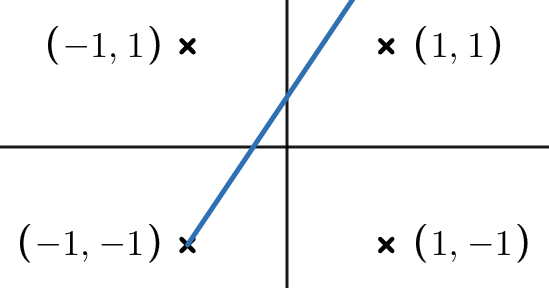
\includegraphics[width=0.5\linewidth]{Figures/DiscreteGradient.png}
    \caption{The optimal direction is indicated by the blue line, so the next state moves in that direction. The next state can be $(1,1)$ in parallel dynamics, whereas in sequential dynamics, it can be $(-1,1)$}
    \label{fig:discrete_gradient}
\end{figure}

\subsection{Sequential dynamics}
Many properties of the Ising model dynamics are obtained using sequential dynamics. In this part of the article, we will focus on this updating rule.

\begin{definition}[Lyapunov's function - \citet{Lyapunov}]
    \label{def:Lypunov}
    Given an autonomous dynamical system $\dot{x} = f(x)$ with equilibrium point $x_0$, a Lyapunov function is a function $V$ such that:
    \begin{itemize}[itemsep=2pt, topsep=10pt]
        \item $V(x) > 0$ with $x\neq x_0$
        \item $V(x_0) = 0$
        \item $\nabla V(x) \cdot f(x) \leq 0$
    \end{itemize}
    If $V$ exists then $x_0$ is stable for Lyapunov.\\ Remark: for a Lyapunov function it holds that $\dot{V}\left(x\right) \leq 0$
\end{definition}

\bigskip\noindent The dynamics of the neural network are a discretization of an autonomous dynamical system. In this subsection, we will refer to the function denoted by $L_{J,h}$ as a Lyapunov function, although this is not a rigorous definition. The following lemma defines this function and relates the interpretation in \cref{fig:discrete_gradient} to the Lyapunov function in \cref{def:Lypunov}.

\begin{lemma}[Decreasing function] \label{lemma:Lyap}
    Using Ising's model with sequential dynamics and interaction $J$ such that $J_{ii} \geq 0$ and $J_{ij}=J_{ji}$, the following function:
    \[
          L_{J,h}(\xi) = -\frac{1}{2} \sum_{ij} \xi_i J_{ij} \xi_j - \sum_{i} h_i \xi_i
    \]
    decreases over time: $L_{J,h}\left(\xi^{\text{new}}\right) \leq L_{J,h}\left(\xi\right)$.

    \begin{proof}
    \noindent Sequential dynamics can change only one value of the network so we can suppose that $i$ is the updated neuron: $\xi_k^{\text{new}} = \xi_k$ for all $k\neq i$.

    \noindent If $\xi_i^{\text{new}} = \xi_i$ there is not any difference, so now we assume $\xi_i^{\text{new}} = -\xi_i$ and study the variation of Lyapunov function $\Delta L_{J,h}$:
    \begin{align*}
         \Delta L_{J,h}\left(\xi,\xi^{\text{new}}\right) &= - \frac12 \sum_{k,l} J_{kl}\left(\xi_k^{\text{new}}\xi_l^{\text{new}} - \xi_k \xi_l\right) - \sum_l h_l \left(\xi_l^{\text{new}}-\xi_l\right) \\
         &\upeq{1} - \sum_{l \neq i} J_{il}\left(\xi_i^{\text{new}}\xi_l^{\text{new}} - \xi_i \xi_l\right) - (-2 h_i\xi_i) \\
         &= - \sum_{l \neq i} J_{il}\left(-\xi_i\xi_l - \xi_i \xi_l\right) - (-2 h_i\xi_i) = 2 \sum_l J_{il} \xi_i \xi_l + 2h_i \xi_i - J_{ii} \\
         &= 2 \xi_i \left( \sum_l J_{il} \xi_l + h_i \right) - J_{ii} \upeq{2} -2\left|\left( \sum_l J_{il} \xi_l +h_i \right)\right| - J_{ii} \leq 0
    \end{align*}
    In equivalence $1$ we used the symmetry of $J$ and $\xi,\xi^{\text{new}} = \pm1$.\\ In equivalence $2$ we used the update formula:
    \[
        \xi_i\left( \sum_l J_{il} \xi_l + h_i \right) = \xi_i\sgn\left[\sum_l J_{il} \xi_l +h_i \right]\left|\sum_l J_{il} \xi_l +h_i \right| = \xi_i\xi_i^{\text{new}}\left|\sum_l J_{il} \xi_l +h_i \right|
    \]
    \end{proof}
\end{lemma}

\begin{remark}[lower bound]
    We can see that the Lyapunov function is lower bounded:
\begin{align*}
    L_{J,h}(\xi) &= -\frac12 \sum_{i,j} \xi_iJ_{ij}\xi_j - \sum_i h_i\xi_i \\
    &\geq -\frac12 \sum_{i,j} J_{ij} - \sum_i h_i \geq -\frac{N^2}{2} |J| - N |h|
\end{align*}
where $|J| = \max_{i,j} |J_{ij}|$ and $|h| = \max_i |h_i|$.

\noindent Through the dynamic of the Ising's model, the value of the Lyapunov function decreases until it reaches a minimum $L^*$.
\end{remark}

\noindent The last step is to find a fixed point of the updating (in sequential dynamic) and to obtain the lower bound at it. In this way we know that the fixed point is stable for Lyapunov. The idea is to choose $J$ and $h$ such that the final configuration of the system is something meaningful. In particular, we want to store $P$ patterns $(x_1,...,x_P)$ in the network and given a starting point $\xi$ retrieve some pattern as the final point of the dynamics. Following this perspective we can interpret the value of the Lyapunov function as an energy function for the system that will evolve towards the minimum points.

\noindent We need to make these patterns the minimum points of the Lyapunov function to do this analysis. This problem can be solved using Hebb's rule:
\begin{definition}[Hebb's rule]
    \label{def:Heb}
    Given $P \leq N$ patterns $(x_1,\ldots,x_P)$ we define Hebbian interaction matrix as:
    \[
    J_{ij} = \frac1N (1 - \delta_{i,j}) \sum_{\mu=1}^P x^{\mu}_i x^{\mu}_j
    \]
\end{definition}
\begin{lemma}[Pattern as minimum points]
   \label{lemma:Heb}
   Let $J$ be made with the Hebbian rule using orthogonal patterns (i.e. $\sum_i x^{\mu}_i x^{\nu}_i =N \delta_{\mu,\nu}$ ), every pattern $x^{\mu}$ is a global minimum for the Lyapunov function with $h=0$.
   \begin{proof}
       \begin{align*}
            L_{J,h}(\xi) &= -\frac12 \sum_{i,j} \xi_i J_{ij} \xi_j  =
            -\frac12 \frac1N \sum_{i,j} (1 - \delta_{i,j}) \sum_{\mu} x^{\mu}_i x^{\mu}_j \xi_i \xi_j \\
            &= -\frac12\frac1N \sum_{i \neq j} \sum_{\mu} x^{\mu}_i x^{\mu}_j \xi_i \xi_j =
            \frac12P  -\frac12\frac1N \sum_{i,j} \sum_{\mu} x^{\mu}_i x^{\mu}_j \xi_i \xi_j = \\
            &= \frac{1}{2}P - \frac{1}{2}\sum_{\mu} \left( \frac{1}{\sqrt{N}} \sum_i x^{\mu}_i \xi_i \right)^2 \geq \frac{1}{2}(P - N) \upeq{1}  L_{J,h}(x^{\nu}) \quad \forall x^{\nu} \in (x_1,\ldots,x_P)
            \end{align*}
            the last inequality holds because of the orthogonality of the patterns with same euclidean norm $N$:
            \[
            \sum_{\mu} \left( \frac{1}{\sqrt{N}} \sum_i x^{\mu}_i \xi_i \right)^2 = \|\xi\|^2 \leq N
            \]
   \end{proof}
\end{lemma}

\subsection{Stochastic model}
With this framework we already use the network for pattern retrieval, but there are two main problems: the first is that the patterns are not always orthogonal, the second is that we can also retrieve a local minimum of the Lyapunov function, to overcome this problem we introduce the stochastic model.

\noindent Assume that $U^\star$ is not a deterministic threshold, and that we can express it in this way:
\[
    \forall{i}\left(U_i^\star\left(t\right) = U_i^\star - \frac12 T z_i\left(t\right)\right)
\]
with $z_i\left(t\right)\sim\mathcal{P}$ such that it's symmetric ($\implies\overline{z_i\left(t\right)}=0$) and $\overline{z_i\left(t\right)^2}=1$. The distribution function of $\mathcal{P}$ is denoted with $g\left(x\right)=\frac12 + \int_0^x\mathcal{P}\left(u\right)du$.

\noindent $T$ is called \textbf{temperature} and is not negative. The temperature controls the randomness of the process: $T=0$ implies a deterministic behaviour and as T increases, the behaviour tends to become increasingly random, approaching completely random behaviour in the limit as $T \to \infty$.

\begin{remark}
   We will use $g\left(x\right)=\frac12\left(1-\tanh\left(x\right)\right)$
\end{remark}

\begin{definition}[Stochastic sequential dynamics]
    \label{def:stocdyn}
    Consistent with the sequential dynamics of the deterministic process, we define the stochastic update using a non-deterministic threshold.

    \noindent Let $U_t\sim \textit{Unif}\left(\left[N\right]\right)$, for each component $i$ it holds that:
    \[ \xi_i^{t+1} \mathdef
    \begin{cases}
        \sgn\left[\phi_i(\xi^t) + Tz_i(t)\right] & \text{if }\;U_{t+1}=i \\
        \xi_i^t & \text{otherwise}
    \end{cases}
    \]
    remark: $z_i$ is a random variable for each $t$.
\end{definition}

\begin{lemma}[stochastic derivation]
    \label{lemma:stoch_der}
    Using an Ising model with sequential dynamics, we can formulate the following thesis:
    \[
        \mathbb{P}\left[\xi^{t+1}=\xi'\middle|\xi^t=\xi\right] =
        \frac{1}{N}\sum_i \frac{1}{2} (1 + \xi'_i \tanh(\beta \phi_i(\xi' )) \delta_{\xi,\xi'} + \frac{e^{-\beta \xi_i \phi_i(\xi)}}{2\cosh(\beta\phi_i(\xi))} \delta_{F_i(\xi),\xi'}
    \]
    where $F_i $ is the flip operator (it changes the sign of the $i^{\text{th}}$ component) and $\beta = \frac{1}{T}$
    \begin{proof}
    We can divide the proof in three cases:
    \begin{itemize}
        \item[i)] $\xi' = \xi$
        \begin{align*}
            &\mathbb{P}\left[\xi^{t+1}=\xi'\middle|\xi^t=\xi\right]
            = \mathbb{P}\left[\xi^{t+1}=\xi\middle|\xi^t=\xi\right]
            = \sum_i \mathbb{P}\left[\xi^{t+1}=\xi\middle|\xi^t=\xi, U_{t+1}=i\right]\mathbb{P}\left[U_{t+1}=i\right] \\
            &= \frac1N \sum_i \mathbb{P}\left[ \sgn\left[\phi_i(\xi^t) + Tz_i(t) \right] = \xi_i\middle|\xi^t=\xi, U_{t+1}=i\right]
            = \frac1N \sum_i \mathbb{P}\left[ \sgn\left[\phi_i(\xi) + Tz_i(t) \right] = \xi_i\right] \\
            &= \frac1N \sum_i \mathbb{P}\left[ \xi_i\left(\phi_i(\xi) + Tz_i\left(t\right) \right) \geq 0 \right]
            \upeq{1} \frac1N \sum_i \mathbb{P}\left[z_i(t) \geq - \beta \xi_i \phi_i\left(\xi\right) \right] \\
            &= \frac1N \sum_i \frac12 \left(1 + \xi_i \tanh\left(\beta \phi_i\left(\xi\right)\right)\right)
        \end{align*}
        In equivalence $1$ we used the relation $\xi_i z_i \sim z_i$ due to the symmetry

        \item[ii)] $\xi' = F_i(\xi)$
        \begin{align*}
            &\mathbb{P}\left[\xi^{t+1}=\xi'\middle|\xi^t=\xi\right]
            = \mathbb{P}\left[\xi^{t+1}=F_i(\xi)\middle|\xi^t=\xi\right] \\
            &= \mathbb{P}\left[\xi^{t+1}=F_i(\xi)\middle|\xi^t=\xi, U_{t+1}=i\right]\mathbb{P}\left[U_{t+1}=i\right] + \mathbb{P}\left[\xi^{t+1}=F_i(\xi)\middle|\xi^t=\xi, U_{t+1}\neq i\right]\mathbb{P}\left[U_{t+1}\neq i\right]\\
            &= \frac{1}{N} \mathbb{P}\left[ \sgn\left[\phi_i(\xi^t) + Tz_i(t) \right] = F_i(\xi)_i\middle| \xi^t=\xi, U_{t+1}=i\right] \\
            &= \frac{1}{N}  \mathbb{P}\left[ \xi_i\left(\phi_i(\xi^t) + Tz_i\left(t\right) \right) \leq 0 \right]
            = \frac{1}{N} \mathbb{P}\left[z_i(t) \leq - \beta \xi_i \phi_(\xi) \right] \\
            &= \frac{1}{2} \left(1 - \xi_i \tanh\left(\beta \phi_i\left(\xi \right)\right)\right) = \frac{e^{-\beta \xi_i \phi_i(\xi)}}{2\cosh(\beta\phi_i(\xi))}
        \end{align*}
        \item[iii)] otherwise\\
        Sequential dynamics can only change one neuron for each update so the probability is $0$.
    \end{itemize}

    \end{proof}
\end{lemma}

\paragraph{Markov chains} In \cref{lemma:stoch_der} we proved that only the last state established the new state. This condition defines a Markov chain over $\{-1,1\}^N$. Define $W_{\xi,\xi'}$ the probability to jump from $\xi$ in $\xi'$:
\[
    W_{\xi,\xi'} =
        \frac{1}{N}\sum_i \frac{1}{2} (1 + \xi'_i \tanh(\beta \phi_i(\xi' )) \delta_{\xi,\xi'} + \frac{e^{-\beta \xi \phi_i(\xi)}}{2\cosh(\beta\phi_i(\xi))} \delta_{F_i(\xi),\xi'}
\]
The matrix $W=\left(W_{\xi,\xi'}\right)_{\xi,\xi'}$ is the transition matrix of the Markov chain.

\begin{remark}
    Recall following properties:
    \begin{itemize}[itemsep=2pt, topsep=5pt]
        \item $\exists\tau\left(t\geq\tau\implies W^t > 0\right)$, so it is an ergodic Markov chain. So there exists a unique invariant distribution $p_{\infty}$ to which the process will converges form any initial state.
        \item If $\forall \xi,\xi'\left(p(\xi) W_{\xi,\xi'} = p(\xi') W_{\xi'\xi}\right)$ then $p$ is an invariant distribution. The equivalence is called \textbf{detailed balance}.
    \end{itemize}
\end{remark}

\noindent We use stochastic dynamics to escape from non-optimal minima. Now we study a limit probability of the state of the neural network using weights $J$ similar to  \cref{def:Heb}. But before addressing the following theorem let us recall this lemma from graph theory.
\begin{lemma}
    \label{lemma:combinatorics}
    Let $G$ graph with vertices $V$ and oriented edges $E$ such that a vertex connected with all vertices exists, called $O$. Each edge $\vec{e}$ has a value $c(\vec{e})$ and $c(-\vec{e}) = -c(\vec{e})$ (it is called '\textit{flux}'). The function $K:V\to\mathbb{R}$ (called potential) is such that $K(v)-K(w)=c(\vec{vw})$ exists if and only for each cycle $\vec{e_1},\ldots,\vec{e_n}$ holds $\sum c(\vec{e_k}) = 0$ (flow conservation).

    \begin{proof}
        If $K$ exists, then it's clear that the summation of values over a cycle is $0$.

        \noindent If flow conservation holds, then for each vertices $v$ we can find a path $\vec{e_1},\ldots,\vec{e_n}$ to $O$ from $v$ with vertices $O=v_0,\ldots,v_n=v$, so:
        \[
        K(v)-K(O) = \sum K(v_{i+1}) - K(v_{i})
        \]
        remark: potential exists at less than a constant.
    \end{proof}
\end{lemma}

\begin{theorem}[Invariant measure] \label{teo:Inv_Mea}
    In a sequential stochastic dynamic without self-interactions, i.e. $J_{ii}=0$, detailed balanced is equivalent to symmetric interactions:
    \[
    J_{ij}= J_{ji} \iff p_\infty(\xi) W_{\xi\xi'} = p_\infty(\xi') W_{\xi'\xi} \quad \forall \xi,\xi'
    \]
    Furthermore, the stationary distribution is:
    \[
    p_{\infty}(\xi) \propto e^{-\beta \mathcal{H}_{J,h}(\xi)}
    \]
    where $\mathcal{H}_{J,h} =  -\frac{1}{2} \sum_{i,j} \xi_i J_{ij} \xi_j - \sum_{i} h_i \xi_i$ (called Hamiltonian function).
    \begin{proof}
        We know that if $p$ verifies the detailed balance and $p$ is a distribution, then $p_\infty=p$. So we are going to start by finding an explicit form of a distribution that verifies detailed balance. We are going to prove that this distribution exists if $J$ is symmetric, and then the opposite (only if $J$ is symmetric).

        \bigskip\noindent At the moment, we are rewriting detailed balance in a simple form. \\ If $\xi'=\xi$ or $\xi'\neq\xi \land \forall i\left(\xi' \neq F_i(\xi)\right)$ the detailed balance holds trivially because we get $0=0$. For each $\xi,\xi'$ such that $\exists i\left(\xi' = F_i(\xi)\right)$, we want to express the detailed balance in a simpler form. Using \cref{lemma:stoch_der}:
        \[
            p_{\infty}(\xi) \frac{e^{-\beta \xi_i \phi_i(\xi)}}{2\cosh(\beta\phi_i(\xi))} = p_{\infty}(\xi') \frac{e^{-\beta \xi'_i \phi_i(\xi')}}{2\cosh(\beta\phi_i(\xi'))}
        \]
        We remark that there's no self-interaction, so:
        \[
            \phi_i(\xi) = \sum_j J_{ij}\xi_j+h_i = \sum_{j\neq i} J_{ij}\xi_j + h_i = \sum_{j\neq i} J_{ij}\xi'_j + h_i = \sum_{j} J_{ij}\xi'_j + h_i = \phi_i ( \xi')
        \]
        This gives us an equivalent form of detailed balance sheet:
        \begin{align}
            \label{tmp:1}
            &\forall \xi,\xi'\left(p_\infty(\xi) W_{\xi\xi'} = p_\infty(\xi') W_{\xi'\xi}\right) \\
            &\iff \forall \xi,\xi',i\left(\xi' = F_i(\xi) \implies p_{\infty}(\xi) e^{-\beta \xi_i \phi_i(\xi)} = p_{\infty}(\xi') e^{-\beta \xi'_i \phi_i(\xi')} \right) \nonumber
        \end{align}

        \bigskip\noindent Now let's try to find a distribution $p$ that verifies the detailed balance. We know that the distribution $p_\infty$ is positive over all states, so our target distribution has to be positive over all states as well. We can write $p$ in exponential form: $p\left(\xi\right)=\exp\left(-\beta K(\xi)\right)$. This simplifies the equivalent form in \cref{tmp:1}.

        \noindent Using \cref{tmp:1}, we can verify detailed balance only over the couples $\xi,\xi'$ such that $\exists i\left(\xi'=F_i\left(\xi\right)\right)$. Simplifying:
        \begin{align*}
            &K(\xi) + \xi_i\phi_i(\xi) = K(\xi') + \xi'_i\phi_i(\xi') \\
            &K(\xi')-K(\xi) = 2\xi_i\phi_i(\xi) = 2\xi_i\left(\sum_l J_{il}\xi_l + h_i\right)
        \end{align*}
        Using \cref{lemma:combinatorics}, it is possible to find an explicit form of $K$ if and only if $2\xi_i\left(\sum_l J_{il}\xi_l + h_i\right)$ is a flux that verifies the flow conservation.

        \noindent We can express the flow conservation with a simpler and equivalent condition.

        \noindent Let $i,j$ be different indices, get a path $\mathcal{P}_1=\left(v,F_i(v),F_j(F_i(v))\right)$, we want that the flux over $\mathcal{P}_1$ to be the same flux over $\mathcal{P}_2 = \left(v,F_j(v),F_i(F_j(v))\right)$:
        \begin{align*}
            \text{flux}\left(\mathcal{P}_1\right) &= 2v_i\left(\sum_l J_{il}v_l + h_i\right) + 2F_i(v)_j\left(\sum_l J_{jl}F_i(v)_l + h_j\right) \\
            &= 2v_i\left(\sum_l J_{il}v_l + h_i\right) + 2v_j\left(\sum_l J_{jl}v_l + h_j - 2J_{ji}v_i\right) \\
            &= 2v_i\left(\sum_l J_{il}v_l + h_i\right) + 2v_j\left(\sum_l J_{jl}v_l + h_j\right) - 2J_{ji}v_jv_i \\
            \text{flux}\left(\mathcal{P}_2\right) &= 2v_j\left(\sum_l J_{jl}v_l + h_i\right) + 2F_j(v)_i\left(\sum_l J_{il}F_j(v)_l + h_i\right) \\
            &= 2v_j\left(\sum_l J_{jl}v_l + h_j\right) + 2v_i\left(\sum_l J_{il}v_l + h_i - 2J_{ij}v_j\right) \\
            &= 2v_j\left(\sum_l J_{jl}v_l + h_j\right) + 2v_i\left(\sum_l J_{il}v_l + h_i\right) - 2J_{ij}v_iv_j
        \end{align*}
        so $\text{flux}\left(\mathcal{P}_1\right) = \text{flux}\left(\mathcal{P}_2\right) \iff J_{ij}=J_{ji}$.

        \noindent The flow does not change when we commute $2$ flips. In a cycle we know that if we have a flip $F_i$ then there is another $F_i$. Using commutation we can remove all flips and so the flux is conservative.

         \noindent We prove that there is a potential at less than a constant, and in order to get a distribution from $K$, it's possible to set a particular potential $K(\xi) + \const$ such that $p$ is a distribution. Now we know that the thesis is true, so we can compute $K$ to prove that $p_{\infty}(\xi) \propto e^{-\beta \mathcal{H}_{J,h}(\xi)}$.

        \noindent Seeing that $K(\xi')-K(\xi) = 2\xi_i(\sum_l J_{il}\xi_l + h_i)$ we recognize the result in \cref{lemma:Lyap}:\\ $K(\xi') - K(\xi) = \Delta L_{J,h}(\xi,\xi')$

        \noindent So a good option for the potential $K$ is:
        \[
            K(\xi) = -\frac12\sum_{ij}\xi_iJ_{ij}\xi_j - \sum_i h_i\xi_i + \const = \mathcal{H}_{J,h}(\xi) + \const
        \]
    \end{proof}
\end{theorem}

\section{Statistical mechanics perspective}
According to \cref{teo:Inv_Mea}, there is a connection between the dynamics of the network and spin models studied in statistical mechanics, since the state of a neuron can be associated with the alignment of an atom in a magnetic field, or its spin. Statistical mechanics, a branch of physics, connects the individual properties of atoms or molecules to macroscopic observable quantities such as temperature and pressure. This framework provides insight into how the collective behavior of many particles gives rise to the thermodynamic properties we observe. Using this approach, we can analyze how the behavior of the system changes in response to changes in its parameters. The key idea is to interpret the state of the system as a mixture of pure states - a probability distribution over these pure states - and to identify the configuration that minimizes a given energy function. Another essential aspect is to determine specific order parameters on which the probability distribution depends; by analyzing these, we can gain insight into the behavior of the entire system.

\begin{definition}
	\label{def:gibbs_stat}
	According to statistical mechanics, we can define a state of a system $\rho$ as a convex combination of the set of pure states $\{\rho^1,\ldots,\rho^{\mathcal{N}} \}$\\
	Given a state $\rho$, we define the following quantities:
	\begin{itemize}
		\item[i)] $U(E,\rho) = \sum_i \rho_i E_i$ \quad\textbf{internal energy}
		\item[ii)] $S(\rho) = -K_B \sum_i \rho_i \log(\rho_i) $ \quad \textbf{Gibbs entropy}
		\item[iii)] $ f(E,\rho,T) = U(E,\rho) - T S(\rho) $ \quad \textbf{free energy}
	\end{itemize}
\end{definition}
\begin{definition}[Gibbs distribution]
    \label{def:GibbsDist}
    The limit distribution given in \cref{teo:Inv_Mea} plays a key role in statistical mechanics. In this setting we can rephrase it as Gibbs distribution: \\
    \[
    \rho_{\beta}(\xi) = \frac{e^{-\frac{\beta E(\xi)}{K_B}}}{Z_{\beta}}
    \]
    where: $Z_\beta = \sum_\xi e^{-\frac{\beta E(\xi)}{K_B}} $ is the normalization factor called \textbf{partition function}.

    \bigskip\noindent In the context of neural networks:
    \begin{itemize}
       \item $E(\xi)=\mathcal{H}_{J,h}(\xi)$ is the energy of the neural network.
       \item $K_B=1$ is a taken factor.
    \end{itemize}
\end{definition}

\noindent The role of this distribution is given by the following theorem:
\begin{theorem}[Gibbs distribution]
     \label{teo:Gibbs}
     The Gibbs distribution is the state $\rho$ where the free energy reaches its minimum, this point is called thermodynamic equilibrium.
     \[
      \inf_\rho f(E,\rho,T) = f(E,\bar{\rho},T) = -K T \log(\bar{Z})
     \]
    where $\bar{\rho}$ is the Gibbs distribution
    \begin{proof}
        The free energy is a convex function with respect to $\rho$ because the energy is affine and the Gibbs entropy is concave, so we can find its minimum by finding the point where $\delta f = 0$ $\forall \rho$ variations.
        Hence we obtain:
        \[
        \begin{cases}
            \delta f = \sum_i E_i\delta\rho_i  + KT(\log(\rho_i)+1)\delta\rho_i \upeq{1} \sum_i (E_i + KT\log(\rho_i))\delta\rho_i = 0 \\
            \sum_i \delta\rho_i = 0
        \end{cases}
        \]
        In equivalence $1$ we use the second equation.

        \noindent From the first equation we can state that $E_i + KT\log(\rho_i)$ must not depend on $i$ because the system must hold for any variation. So we can say that if $\bar{\rho}$ exists then:
        \[
        E_i + KT\log(\bar{\rho_i}) = \bar{F}
        \]
        from which we get $\bar{\rho_i}$, we have:
        \[
        \bar{\rho}_i = e^{-\frac{E_i-\bar{F}}{KT}}
        \]
        The constant $\bar{F}$ must be taken to satisfy:
        \[
         1=\sum_i \bar{\rho}_i = \sum_i e^{-\frac{E_i-\bar{F}}{KT}} = e^{\frac{\bar{F}}{KT}}\sum_i e^{-\frac{E_i}{KT}}
        \]
        \noindent Using the definition of free energy and the formula for $\bar{\rho}$ we obtain:
        \begin{equation}
            f(E,\bar{\rho},T) = \bar{F}e^{\frac{\bar{F}}{KT}}\sum_i e^{-\frac{E_i}{KT}} = \bar{F}
        \end{equation}
        We can state that $\bar{Z} = e^{-\frac{\bar{F}}{KT}}$.
    \end{proof}
\end{theorem}

\bigskip\noindent We introduced noise to escape unwanted local minima, but in this way it is not possible to assume that the sequence converges to ideal states. So we found the limit distribution and observed that it is the Gibbs distribution (see \cref{teo:Inv_Mea}).

\noindent As the sequential deterministic dynamics reduces the Lyapunov function (see \cref{lemma:Lyap}), the sequential stochastic dynamics reduces the free energy. However, the convergence is towards the optimal density (see \cref{teo:Gibbs}).

\subsection{Curie-Weiss model}
To introduce the way of working of statistical mechanics, we begin with an analysis of the Curie-Weiss model.
\begin{definition}[Curie-Weiss model]
	The Curie-Weiss model is an Ising model in which the Hamiltonian function is:
	\[
	\mathcal{H}_{N,J,h}(\xi) = - \sum_{i\neq j} \frac{J}{2} \xi_i \xi_j - h \sum_i \xi_i
	\]
	Note: This is a special case where $J_{ii}=0$, $J$ symmetric and $J_{ij}$ is constant where $i\neq j$.
\end{definition}
This type of model is called a mean field model because each neuron interacts with all the others in the same way. The goal of the analysis here is to understand the behavior of the magnetization.
\begin{definition}[magnetization]
	Given a state $\xi$ we call the magnetization the quantity:
	\[
	m_N(\xi) = \frac{1}{N} \sum_i \xi_i
	\]
\end{definition}
The magnetization is what we call an observable quantity because it depends on the state of all the neurons, not just one. An important observation is that we can write the Hamiltonian as a function of the magnetization as:
\[
	\mathcal{H}_{N,J,h}(\xi) = - \frac{NJ}{2} m_N(\xi)^2 - h N m_N(\xi)
\]
We know thanks to the \cref{teo:Gibbs} that the distribution that minimizes the free energy is the observed one, but we don't know anything about the magnetization, so our goal is to understand how it is effected by the temperature, at least when $N$ is very large. Taking $N \to \infty$ is a key concept in statistical mechanics and it is called thermodynamic limit (TDL) it allows us to simplify some calculations by removing the dependence from the size of the model. To calculate the thermodynamic limit, we need to recall and introduce some quantities:
\begin{definition}[Curie-Weiss quantities]
\label{def:CWqt}
We define quantities for Curie - Weiss model:
    \begin{itemize}
        \item $\rho_{N,\beta,J,h}(\xi) =\frac{ e^{-\beta \mathcal{H}_{N,J,h}(\xi)}}{Z_{N,\beta,J,h}} $ \quad \textbf{equilibrium distribution}
        \item $Z_{N,\beta,J,h} $ \quad \textbf{partition function}
        \item $F_{N,\beta,J,h} = -\frac{1}{\beta } \log(Z_{N,\beta,J,h}) $ \quad \textbf{free energy}
        \item $f_{N,\beta,J,h} = -\frac{1}{\beta N} \log(Z_{N,\beta,J,h}) $ \quad \textbf{intensive free energy}
        \item $f_{\beta,J,h} = \lim_{N \to \infty} f_{N,\beta,J,h}$ \quad \textbf{intensive free energy in TDL}
    \end{itemize}

	\bigskip\noindent Note: These definitions are addressed with definitions in \cref{def:gibbs_stat} using the Gibbs distribution $\bar{\rho}$.
\end{definition}
Now we are ready to analyze the Curie-Weiss model.

\noindent First, we will try to understand the probability distribution of the magnetization when the states follow the equilibrium distribution (\cref{def:GibbsDist}):
\[
\rho_{N,\beta,J,h}(m) \mathdef \mathbb{P}_{\xi\sim\bar{\rho}}\left[m_N(\xi) = m\right] = \sum_{\xi}  \rho_{N,\beta,J,h}(\xi) \delta(m_N(\xi) = m )
\]
This measure is called \textbf{coarse grained measure} and our goal is to understand how it relates to the equilibrium measure in the TDL.\\
We also introduce the coarse-grained partition function, which is
\[
Z_{N,\beta,J,h}(m) \mathdef \sum_{\xi} e^{-\beta \mathcal{H}_{N,J,h}(\xi)} \delta(m_N(\xi) = m )
\]
\begin{definition}[coarse grained measure] We will continue these definitions with other coarse-grained partition functions:
    \begin{itemize}
        \item $\rho_{N,\beta,J,h}(m) = \sum_{\xi}  \rho_{N,\beta,J,h}(\xi) \delta(m_N(\xi) = m ) $ \quad \textbf{probability magnetisation}
        \item $Z_{N,\beta,J,h}(m) = \sum_{\xi} e^{-\beta \mathcal{H}_{N,J,h}(\xi)}  \delta(m_N(\xi) = m ) $ \quad \textbf{partition function}
        \item $F_{N,\beta,J,h}(m) = -\frac{1}{\beta } \log(Z_{N,\beta,J,h}(m)) $ \quad \textbf{free energy}
        \item $f_{N,\beta,J,h}(m) = -\frac{1}{\beta N} \log(Z_{N,\beta,J,h}(m)) $ \quad \textbf{intensive free energy}
        \item $f_{\beta,J,h}(m) = \lim_{N \to \infty} f_{N,\beta,J,h}(m)$ \quad \textbf{intensive free energy in TDL}
\end{itemize}
\end{definition}

\begin{proposition}
    Using this formalism we can express the probability of the magnetization from the intensive free energy in TDL:
    \begin{align}
        \rho_{N,\beta,J,h}(m) &= \sum_{\xi}\frac{ e^{-\beta \mathcal{H}_{N,J,h}(\xi)}  \delta\left(m_N(\xi)
        = m\right)}{Z_{N,\beta,J,h}}
        = \frac{Z_{N,\beta,J,h}(m)}{Z_{N,\beta,J,h}} \nonumber \\
        &= \frac{\exp\left(\frac{\beta}{\beta}\log\left(Z_{N,\beta,J,h}\left(m\right)\right)\right)}{\exp\left(\frac{\beta}{\beta}\log\left(Z_{N,\beta,J,h}\right)\right)}
        = \frac{\exp\left(-\beta F_{N,\beta,J,h}(m)\right)}{\exp\left(-\beta F_{N,\beta,J,h}\right)}
        = e^{-\beta(F_{N,\beta,J,h}(m)-F_{N,\beta,J,h})} \nonumber \\
        &= e^{-\beta N \left(f_{N,\beta,J,h}(m)-f_{N,\beta,J,h}\right)} \label{eq:Z_m_sum}
    \end{align}
\end{proposition}
\begin{remark}
    In this way we can calculate the initial definitions in \cref{def:CWqt} in terms of intensive free energy in TDL:
    \begin{align}
        Z_{N,\beta,J,h} &= \sum_\xi \rho_{N,\beta,J,h}(\xi) = \sum_m \sum_\xi \rho_{N,\beta,J,h}(\xi)  \delta(m_N(\xi) = m ) \nonumber \\
        &= \sum_m  Z_{N,\beta,J,h}(m) = \sum_m e^{-\beta N f_{N,\beta,J,h}(m)}
    \end{align}
\end{remark}

\noindent This formulation suggests that the terms that most influence the partition function are those where the value of $f_{N,\beta,J,h}(m)$ is minimized. Moreover, if $f_{\beta,J,h}(m)$ has a minimum in $m^*$, we can state for the thermodynamic limit, using the Taylor expansion for $f_{\beta,J,h}(m)$, that
\begin{align*}
    \lim_{N\to\infty}Z_{N,\beta,J,h} &\upeq{1}  \lim_{N\to\infty}\sum_m e^{-\beta N f_{N,\beta,J,h}(m)} = \lim_{N\to\infty} \int_{-\infty}^{+\infty}  e^{-\beta N f_{\beta,J,h}(m)}dm \\
    &=\lim_{N\to\infty} \int_{-\infty}^{+\infty} e^{-\beta N\left(f_{\beta,J,h}(m^*) + \frac{f''_{\beta,J,h}(m^*)(m-m^*)^2}{2} \right)}dm\\
    &= \lim_{N\to\infty}e^{-\beta N f_{\beta,J,h}(m^*) } \sqrt{\frac{2\pi}{N\beta f''_{\beta,J,h}(m^*)}}
\end{align*}
Where in the equivalence $1$ we used a similar conclusion of \cref{eq:Z_m_sum}, using this relation within the definition of the intensive free energy in TDL we get:
\begin{align*}
    f_{\beta,J,h} &= \lim_{N \to \infty}  -\frac{1}{\beta N} \log(Z_{N,\beta,J,h})  \\
    &= \lim_{N \to \infty}  -\frac{1}{\beta N} \log\left(e^{-\beta N f_{\beta,J,h}(m^*) } \sqrt{\frac{2\pi}{N\beta f''_{\beta,J,h}(m^*)}} \right)\\
    &=  \lim_{N \to \infty} -\frac{-\beta N  f_{\beta,J,h}(m^*)}{\beta N}  -\frac{\log\left(\sqrt{\frac{2\pi}{N\beta f''_{\beta,J,h}(m^*)}} \right)}{\beta N}\\
    &=  \lim_{N \to \infty} f_{\beta,J,h}(m^*) =  f_{\beta,J,h}(m^*)
\end{align*}
So if we can find the minima of the intensive free energy for each $N$ ($m^\star_N$) and then we would like to be able to compute all minima $m^\star$ and thus the intensive free energy for TDL.

\bigskip\noindent From \cref{teo:Gibbs} we know that we can express intense free energy as
\[
     f_{N,\beta,J,h}(m) = \frac{E_{N,\beta,J,h}(\rho_{N,\beta,J,h}(m)) - T S(\rho_{N,\beta,J,h}(m))}{N}
\]
We consider only the configuration with a fixed magnetization, so the energy is constant and the distribution is uniform over the number of possible configurations, which allows us to say:
\[
    f_{N,\beta,J,h}(m) = \frac{- \frac{NJ}{2} m^2 - h N m}{N} - T \frac{S(\text{Unif}\left[\Omega_N(m)\right]))}{N} = - \frac{J}{2} m^2 - h  m +
    T \frac{\log(\Omega_N(m))}{N}
\]
where $\Omega_N(m) = \sum_\xi \delta(m(\xi)-m)$ is the number of possible configurations.

\noindent In the TDL we get
\begin{align*}
	f_{\beta,J,h}(m) =& \lim_{N\to \infty} f_{N,\beta,J,h}(m) = - \frac{J}{2} m^2 - h m + \lim_{N\to \infty} T \frac{\log(\Omega_N(m))}{N}\\ =& - \frac{J}{2} m^2 - h m + T\left[\frac{1+m}{2} \log\left(\frac{1+m}{2} \right) + \frac{1-m}{2} \log\left(\frac{1-m}{2} \right) \right]
\end{align*}
We are interested in finding the minimum so that we can take the derivative:
\[
f'_{\beta,J,h}(m) = -J m -h + T \left[\frac12 \log\left(\frac{1+m}{1-m} \right) \right] =
-J m -h + T \tanh^{-1}(m)
\]
So stationary points are characterized by the following equation:
\begin{equation}
	\label{eq:Sel_const_CW}
	m^* = \tanh(\beta (Jm^* + h))
\end{equation}
This relation is called the self-consistent equation for the Curie-Weiss model and we can't solve it analytically. We will analyze it when $h=0$ to understand where the minimum of the free energy is. \\
The first observation is that $m^*= 0$ is always a solution and we can find the solution graphically. In a Cartesian graph with the axis $x,y$ we draw the line $\left\{(x,y) \middle| y = x\right\}$ and the function $\left\{(x,y)\middle | y = \tanh(\beta (Jm^*)\right\}$. \\
\begin{figure}[!ht]
    \centering
    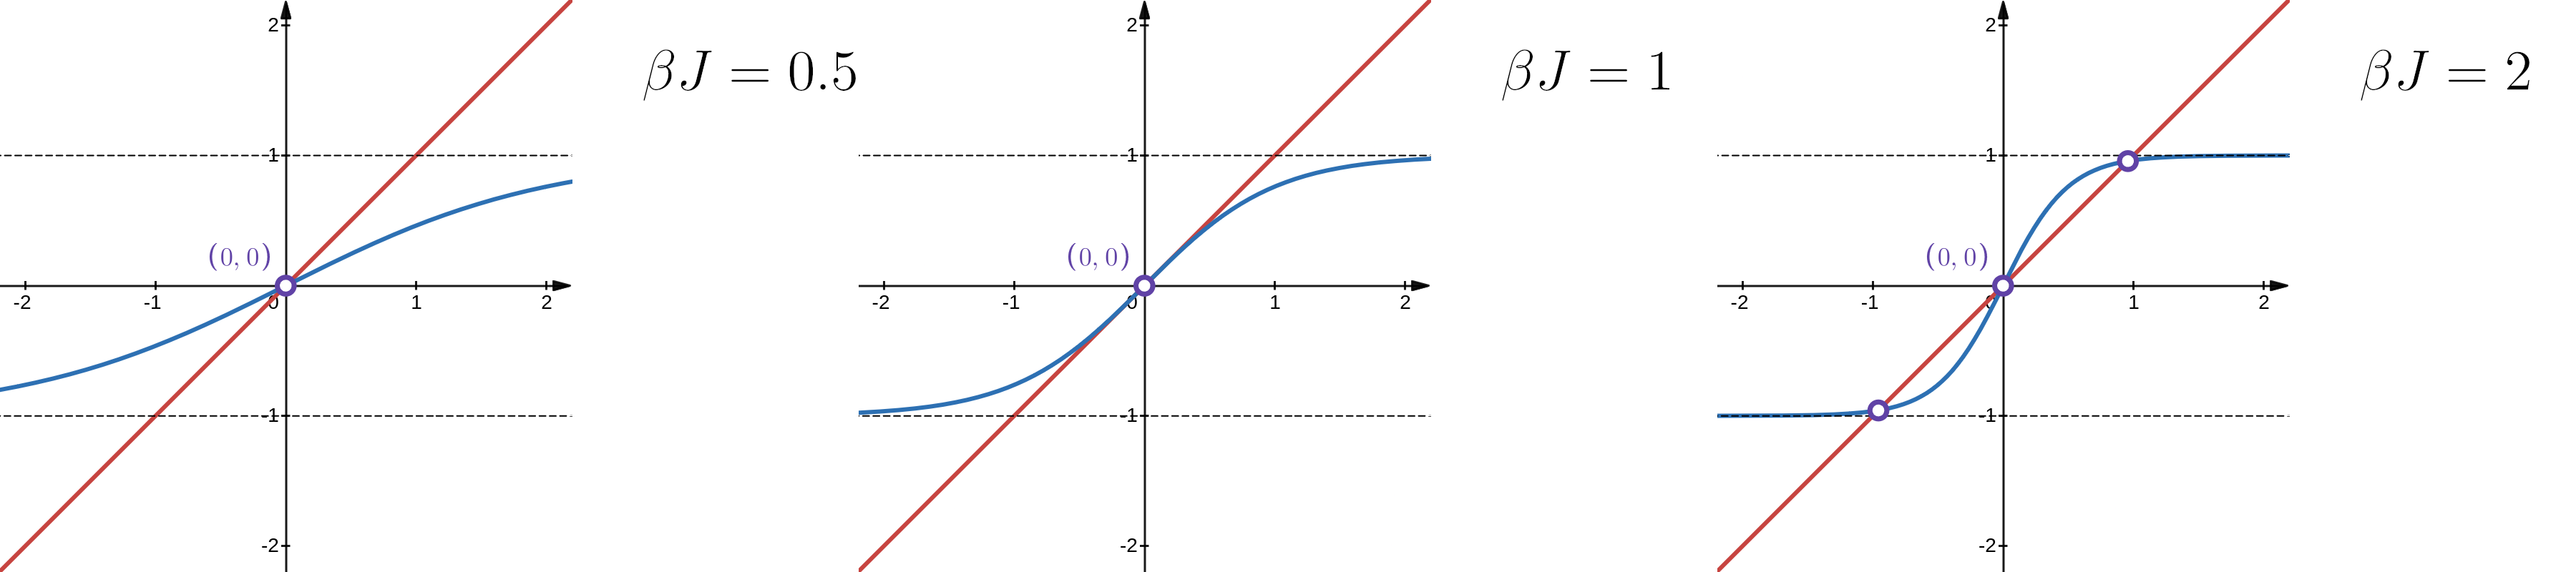
\includegraphics[width=1.0\linewidth]{Figures/3graphs.png}
\end{figure}
\bigskip\noindent We want to understand when the \cref{eq:Sel_const_CW} has one solution and when it has three solutions. To do this, we will analyze the derivative of $\tanh(\beta (Jm)$ in zero:
\[
   \frac{d\tanh(\beta Jm)}{dm}\bigg|_{m=0} = (1- \tanh^2(\beta Jm))\beta J \bigg|_{m=0} = \beta J
\]
From this we can see that the equation has one solution if $\beta J \leq 1$ and three solutions if $\beta J> 1$. \\
Now, from the graph of the free energy in both cases, we can see that $m^*= 0$ is a minimum if $\beta J \leq 1$ and that the positive and negative solutions are minima if $\beta J > 1$.\\
\begin{figure}[!ht]
    \centering
    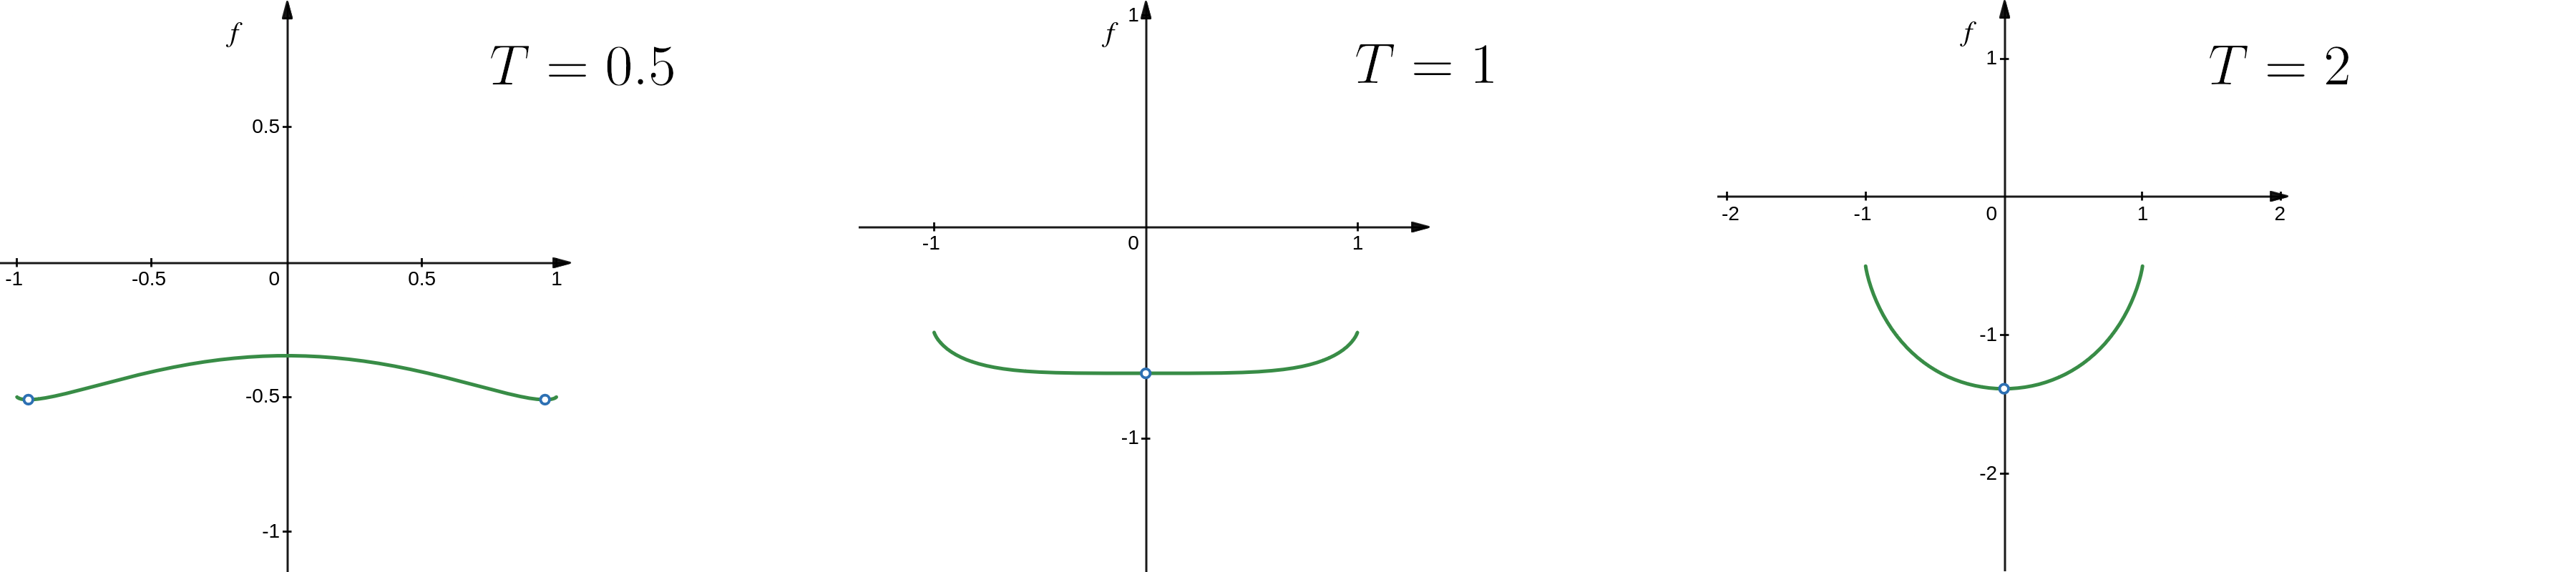
\includegraphics[width=1.0\linewidth]{Figures/3graphsE.png}
\end{figure}

The behavior of the system is completely different in the two cases divided by the critical temperature $T_c = J$, in fact for temperatures above $T_c$ randomness prevails and there are only disordered states, instead for temperatures lower than $T_c$ ordered states appear.  \\
Now we want to analyze the magnetization as a function of temperature to understand its behavior near the critical temperature.

\noindent To do this we will use the Taylor expansion of the hyperbolic tangent inside the \cref{eq:Sel_const_CW}:
\[
    m = \beta J m - \frac13 (\beta J m )^3 + o(m^5)
\]
Ignoring the higher order terms, we can find the solutions as follows:
\[
 m^* = \pm \sqrt{\frac{3(\beta J - 1)}{(\beta J)^3}} = \pm \sqrt{\frac{3(T_c-T)}{T_c (\beta J)^2}} \sim \sqrt{T_c-T}
\]
So we can conclude that the solution can be represented as a continuous function with a discontinuous derivative. \\ From this model we can understand two key concepts of statistical mechanics:
\begin{itemize}
	\item \textbf{Phase transition}\\
	We have seen that the magnetization can be written as a function of temperature and that this function has a
	discontinuous derivative. This phenomenon suggests that the model is in a completely different state depending on the temperature, just as different materials can be gas, solid and liquid. In statistical mechanics this type of behavior is called a phase transition and it is associated with a discontinuity of a derivative of the free energy.
	\item \textbf{Ergodicity breaking}\\
	In the previous setting we noticed that the Markov chain representing the dynamics of the model is ergodic, so it is possible to replace the space average of a quantity with infinite time average along the trajectory for any starting configuration instead in the TDL different starting point gives different result if the temperature is less than the critical temperature.
	This is only possible in TDL and makes the system no longer invariant to its symmetries (in CW a symmetry is given by flipping all neurons). This is something we want to transport into a neural network to get different results with different initial conditions.
\end{itemize}
The last question about the Curie-Weiss model is how it relates to the neural network we defined previously. To understand this connection, we consider a network with a single stored pattern $x$, $h=0$ and the interaction matrix $J$ built with \cref{def:Heb}. We get the following Hamiltonian
\[
\mathcal{H}_{N,J}(\xi) = - \sum_{i,j} J_{i,j} \xi_i \xi_j = - \frac{1}{N} \sum_{i\neq j} (\xi_i x_i)(\xi_j x_j) = - N m_{N,x}(\xi)^2
\]
where $m_{N,x}(\xi) = \frac{1}{N} \sum_i \xi_i x_i $ \quad \textbf{Mattis magnetization}\\
So it is equivalent to a Curie-Weiss model where $J = 2$.\\
Given an initial state, we can use as output the Mattis magnetization after a sufficient number of updates. We can affirm that with a large enough number of neurons (so we can use TDL as a good approximation) and a low temperature, the system will evolve to show a magnetization close to the chosen pattern. It is important to note that there are two main attractors in this type of system, one related to the actual pattern ($m_{N,x}(\xi) \approx 1$) and the other with its negative ($m_{N,x}(\xi) \approx -1$), so this simple network gives as output the pattern or its negative, depending on which is "closer" to the initial configuration.
\subsection{Hopfield model}
In the previous pages we analyzed a network that stores one pattern, now we want to understand networks with more patterns, so we try again to express the Hamiltonian as a function of some order parameter.
\begin{definition}[Mattis magnetizzation] \label{def:mattis_mgn}
Given the patterns $(x^1,\ldots,x^P)$ and a state $\xi$ we define:
\[
    m_{N,\mu}(\xi) = \frac{1}{N} \sum_i  \xi_i x^\mu_i \quad \forall \mu \in \{1,\ldots,P\}
\]
\end{definition}
This definition allows us to write the Hamiltonian with $J$ defined by the Hebb's rule (see \cref{def:Heb}) as:
\[
    \mathcal{H}_{N,X}(\xi)  = \frac12 \sum_{i,j} \frac1N (1 - \delta_{i,j}) \sum_{\mu=1}^P x^{\mu}_i x^{\mu}_j \xi_i \xi_j =
    -\frac{N}{2} \sum_\mu  m_{N,\mu}(\xi)^2
\]
As we defined before $P \leq N$ and $X \in \mathbb{R}^{N \times P}$ is the design matrix. As before we are interested in the analysis of the system in the TDL and we can have two cases:
\begin{itemize}
    \item \textbf{low load regime} where $\lim_{N\to\infty} \frac{P}{N} = 0$
    \item \textbf{high load regime} where $\lim_{N\to\infty} \frac{P}{N} > 0$
\end{itemize}
We will analyze the low load regime. We already know that the free energy can be expressed as the logarithm of the partition function, but with this method we do not remove the dependence of the free energy on the patterns $X$. To remove this dependence we need to define the concept of quenched free energy:
\begin{definition}[Quenched free energy]
We define the quenched free energy as the average over all possible pattern realizations of the free energy:
\begin{itemize}
    \item $Z_{N,\beta,X} = \sum_\xi e^{-\beta\mathcal{H}_{N,X}\left(\xi\right)}$ \textbf{partition function}
    \item $f_{N,\beta,X} = -\frac{1}{N\beta}\log\left(Z_{N,\beta,X}\right)$ \textbf{intensive free energy}
    \item $f_{\beta,X} = \lim_{N\to\infty} f_{N,\beta,X}$
    \item $f^Q_{N,\beta} = \mathbb{E}\left[f_{N,\beta,X}\right] = -\frac{1}{\beta N} \frac{1}{2^{N\times P}}\sum_{X \in \mathbb{R}^{N \times P}}\log( Z_{N,\beta,X}) $
    \quad \textbf{intensive quenched free energy}
    \item $f^Q_{\beta}= \lim_{N \to \infty} f^Q_{N,\beta}  $ \quad \textbf{intensive quenched free energy in TDL}
\end{itemize}
\end{definition}
In the previous definition it is important that the averaging is done before the TDL, in fact it is not true that we can invert these operations.\\
\begin{remark}
    To compute the TDL, we use the Fourier representation of the Dirac delta, i.e:
    \[
    f(x) =\frac{1}{2\pi} \int_{-\infty}^{+\infty} \int_{-\infty}^{+\infty} e^{ik(x-y)} f(y) dy dk
    \]
\end{remark}
\begin{remark}
    To compute the TDL, we use the Laplace's method for approximating integrals:
    \[
    \int_a^b \ldots \int_a^b e^{Nf(z)} dz \subapprox{N\to\infty} \left(\frac{2\pi}{N|-Hf(z^\star)|} \right)^{\frac{P}{2} }e^{Nf(z^\star)}
    \]
    where $f$ is a holomorphic function, $z^\star \in \mathbb{C}^P$ with $P\ll N $ (so we can only use it in the low load regime) is a saddle point for $f$ and the path of the integral passes through $z^\star$, $Hf\left(z^\star\right)$ the Hessian of $f$ in $z^\star$, $\left|-Hf\left(z^\star\right)\right|$ the determinant of $-Hf\left(z^\star\right)$.  \\
    We use this result with $a= -\infty$ and $b=+\infty$

    \noindent It is noted that the approximation is over the difference, so the difference between two members goes to $0$ when $N\to\infty$.
\end{remark}
To compute the quenched TDL, we start from an alternative formulation for the partition function obtained with the Fourier representation of the Dirac delta:
\begin{align*}
    Z_{\beta,N,X} &= \sum_\xi e^{-\beta \mathcal{H}_{N,X}(\xi)} =  \sum_\xi \prod_\mu e^{\frac{\beta N}{2}  m_{N,\mu}(\xi)^2 } \\
    &=  \sum_\xi \prod_\mu \int_{-\infty}^{+\infty} \int_{-\infty}^{+\infty} \frac{1}{2\pi} e^{ik_\mu (m_{N,\mu}(\xi) - y_\mu)} e^{\frac{\beta N}{2} y_\mu^2 }  dy_\mu dk_\mu \\
    &= \sum_\xi  \prod_\mu \int_{-\infty}^{+\infty} \int_{-\infty}^{+\infty}  \left(\frac{ dy_\mu dk_\mu }{2\pi} \right) \exp\left( \frac{i}{N} \sum_j k_\mu x^\mu_j \xi_j - i k_\mu y_\mu + \frac{\beta N}{2} y_\mu^2  \right) \\
    \intertext{We can substitute $k_\mu$ with $\frac{k_\mu}{N}$ and multiply the differential by N }
    &= \sum_\xi  \prod_\mu \int_{-\infty}^{+\infty} \int_{-\infty}^{+\infty}  \left(\frac{ Ndy_\mu dk_\mu }{2\pi} \right) \exp\left( i \sum_{j} k_\mu x^\mu_j \xi_j - iN  k_\mu y_\mu + \frac{\beta N}{2}  y_\mu^2  \right) \\
    \intertext{This formulation allows us to sum over the configurations because we have linear dependence on the argument of the exponential, hence recalling that $\cos(x) = \frac{e^{ix} + e^{-ix}}{2}$ we obtain:}
    &= \int_{\mathbb{R}^{P\times 2}}\prod_\mu \left(\frac{ Ndy_\mu dk_\mu }{2\pi} \right) \exp\left(- iN  \sum_\mu k_\mu y_\mu + \frac{\beta N}{2} \sum_\mu y_\mu^2 \right) \sum_{\xi} \prod_j\prod_\mu\exp\left( i k_\mu x^\mu_j \xi_j\right) \\
    &\upeq{1} \int_{\mathbb{R}^{P\times 2}}\prod_\mu \left(\frac{ Ndy_\mu dk_\mu }{2\pi} \right) \exp\left(- iN  \sum_\mu k_\mu y_\mu + \frac{\beta N}{2} \sum_\mu y_\mu^2 \right) \prod_j\sum_{\xi_j}\prod_{\mu}\exp\left( i k_\mu x^\mu_j \xi_j\right) \\
    &\upeq{2} \int_{\mathbb{R}^{P\times 2}}\prod_\mu \left(\frac{ Ndy_\mu dk_\mu }{2\pi} \right) \exp\left(- iN  \sum_\mu k_\mu y_\mu + \frac{\beta N}{2} \sum_\mu y_\mu^2 \right) \prod_j\left(2\cos\left(\sum_\mu k_\mu x_j^\mu\right)\right) \\
    &= \int_{\mathbb{R}^{P\times 2}} \prod_\mu \left(\frac{N dy_\mu dk_\mu }{2\pi} \right) \exp\left(  \sum_j \log\left(2 \cos\left(\sum_\mu k_\mu x^\mu_j  \right)\right) -i N  \sum_\mu k_\mu y_\mu +  \frac{\beta N}{2} \sum_\mu y_\mu^2  \right) \tag{1}\label{eqHop1}
    \intertext{In equivalence $1$, we used following state:}
    & \sum_\xi\prod_j s_j(\xi_j) = \sum_{\xi_N}\sum_{\xi_1,\ldots,\xi_{N-1}}s_N(\xi_N)\prod_{j=1}^{N-1} s_j(\xi_j) = \sum_{\xi_N}s_N(\xi_N) \sum_{\xi_1,\ldots,\xi_{N-1}}\prod_{j=1}^{N-1}s_j(\xi_j) \\
    & \sum_\xi\prod_j s_j(\xi_j) = \sum_{\xi_N}s_N(\xi_N) \sum_{\xi_1,\ldots,\xi_{N-1}}\prod_{j=1}^{N-1}s_j(\xi_j) = \cdots = \prod_j \sum_{\xi_j}s_j(\xi_j)
    \intertext{In equivalence $2$, we used $\forall j(\xi_j=\pm1)$}
    \intertext{Now we can use the Laplace's method to approximate the integrals, at first, we compute the integral with reference to $y=\left(y_1,\ldots,y_P\right)$. In particular we analyze the problem:}
    &\int_{\mathbb{R}^P} dy \exp\left(N\left( -i  \sum_\mu k_\mu y_\mu +  \frac{\beta}{2} \sum_\mu y_\mu^2\right)  \right)\\
    & \\
    & f(y)\mathdef -i  \sum_\mu k_\mu y_\mu +  \frac{\beta}{2} \sum_\mu y_\mu^2 \\
    & \nabla_y f(y) = \left(-ik_\mu + \beta y_\mu\right)_\mu \\
    & y^\star=\left(\frac{ik_\mu}{\beta}\right)_\mu \tag{2}\label{extr1}\\
    & f(y^\star) = -i  \sum_\mu k_\mu \frac{ik_\mu}{\beta} +  \frac{\beta}{2} \sum_\mu \left(\frac{ik_\mu}{\beta}\right)^2 = \frac{1}{\beta} \sum_\mu \frac{k_\mu^2}{2} \\
    & H_yf(y)\big|_{y^\star} = \left(\beta\delta_{\mu,\nu}\right)_{\mu\nu}\big|_{y^\star}=\beta\mathds{1}_{P} \\
    & \int_{\mathbb{R}^P} dy \exp\left(N\left( -i  \sum_\mu k_\mu y_\mu +  \frac{\beta}{2} \sum_\mu y_\mu^2\right)  \right) \subapprox{N\to\infty} \left(-\frac{2\pi}{N\beta}\right)^{\frac{P}{2}}\exp\left(N \sum_\mu \frac{k_\mu^2}{2\beta}\right) \\
    \intertext{Now we can replace the first integral in \cref{eqHop1} obtaining:}
    & (\ref{eqHop1}) \subapprox{N\to\infty} \left(-\frac{N}{2\pi\beta}\right)^{\frac{P}{2}}\int_{\mathbb{R}^{P\times 2}} dk \exp\left( \sum_j \log\left(2 \cos\left(\sum_\mu k_\mu x^\mu_j  \right)\right) + N \sum_\mu \frac{k_\mu^2}{2\beta}\right)\tag{3}\label{eqHop2} \\
    \intertext{Now we can use the Laplace's method to approximate the integrals with reference to $k=\left(k_1,\ldots,k_P\right)$. In particular we analyze the problem:}
    & \int_{\mathbb{R}^{P\times 2}} dk \exp\left( N\left(\frac1N \sum_j \log\left(2 \cos\left(\sum_\mu k_\mu x^\mu_j  \right)\right) + \sum_\mu \frac{k_\mu^2}{2\beta}\right)\right) \\
    & \\
    & f(k) = \frac{1}{N}\sum_j \log\left(2 \cos\left(\sum_\mu k_\mu x^\mu_j  \right)\right) + \sum_\mu \frac{k_\mu^2}{2\beta} \\
    & \nabla f(k) = \left(-\frac{1}{N}\sum_j \tan\left(\sum_\mu z_\mu x^\mu_j\right)x_j^\nu + \frac{k_\nu}{\beta}\right)_\nu \\
    \intertext{$k^\star$ satisfies:}
    & \forall\nu\left(k_\nu^\star = \frac{\beta}{N}\sum_j \tan\left(\sum_\mu k_\mu^\star x_j^\mu\right)x_j^\nu\right)\tag{4}\label{extr2} \\
    & f(k^\star) = \frac{1}{N}\sum_j \log\left(2 \cos\left(\sum_\mu k_\mu^\star x^\mu_j  \right)\right) + \sum_\mu \frac{\left(k_\mu^\star\right)^2}{2\beta} \\
    \intertext{Now we can replace the approximation in \cref{eqHop2} obtaining:}
    & (\ref{eqHop2}) \subapprox{N\to\infty} \left(\frac{1}{\beta|Hf(k^\star)|}\right)^{\frac{P}{2}}\exp\left(\sum_j \log\left(2 \cos\left(\sum_\mu k_\mu^\star x^\mu_j  \right)\right) + N \sum_\mu \frac{\left(k_\mu^\star\right)^2}{2\beta}\right)\\
    \intertext{We would like, using \cref{extr1}, to write \cref{extr2} and $f(k^\star)$ respect $y^\star \mathdef \frac{i}{\beta}k^\star$: }
    & \forall\nu\left(-i\beta y_\nu^\star = \frac{\beta}{N}\sum_j\tan\left(-i\beta\sum_\mu y_\mu^\star x_j^\mu\right)x_j^\nu\right) \\
    & \iff \forall\nu\left(y_\nu^\star = \frac{1}{N}\sum_j\tanh\left(\beta\sum_\mu y_\mu^\star x_j^\mu\right)x_j^\nu\right) \tag{5}\label{eq:Sel_const_H}\\
    & f(k^\star) = \frac{1}{N}\sum_j \log\left(2 \cos\left(-i\beta\sum_\mu y_\mu^\star x^\mu_j  \right)\right) - \sum_\mu \frac{\beta \left(y_\mu^\star\right)^2}{2} \\
    & \hspace{1.3cm} = \frac{1}{N}\sum_j \log\left(2 \cosh\left(\beta\sum_\mu y_\mu^\star x^\mu_j  \right)\right) - \sum_\mu \frac{\beta \left(y_\mu^\star\right)^2}{2}
    \intertext{now we can express \cref{eqHop2} respect $y^\star$:}
    &(\ref{eqHop2}) \subapprox{N\to\infty} \left(\frac{1}{\beta|Hf(k^\star)|}\right)^{\frac{P}{2}} \exp\left(\sum_j \log\left(2 \cosh\left(\beta\sum_\mu y_\mu^\star x^\mu_j  \right)\right) - N\sum_\mu \frac{\beta \left(y_\mu^\star\right)^2}{2}\right)
    \end{align*}
Now we are ready to calculate the TDL of the free energy:
\begin{align*}
    f_{\beta,X}&= \lim_{N \to \infty} f_{N,\beta,X} =
    \lim_{N \to \infty} -\frac{1}{\beta N} \log( Z_{N,\beta,X})  \\
    &=  \lim_{N \to \infty}  -\frac{1}{\beta N}  \sum_j \log\left(2 \cosh\left(\beta \sum_\mu   y_\mu^\star x_j^\mu \right)\right) + \sum_\mu \frac{(y_\mu^\star)^2}{2} \\
\end{align*}

\begin{theorem}[Quenched free energy low load regime]
\label{teo:HopfreeEnerLR}
    The quenched free energy of the Hopfield model in TDL is:
    \begin{equation}
    \label{eq:FE_Hop}
        f^Q_{\beta} = \frac12 \sum_\mu  (m^*_\mu)^2 -\frac{1}{\beta} \mathbb{E}\left[\log\left(2 \cosh\left(\beta \sum_\nu   m^*_\nu x^\nu \right)\right)\right]
    \end{equation}
         where $m^*$ satisfy the self consistent equations:
    \begin{equation}
    m^*_\mu =\mathbb{E} \left[x^\mu  \tanh\left( \beta  \sum_\nu m^*_\nu x^\nu \right)  \right] \label{eq:SC_Hop}
    \end{equation}
    remark: this notation is justified by \cref{eq:Sel_const_CW} and \cref{eq:Sel_const_H}.
\end{theorem}
We can write the self consistent equation in a vector notation as:
\[
m = \mathbb{E}(X \tanh(\beta m \cdot X))
\]
Moreover, if there is a single pattern to store, we obtain the self-consistent equation for the Curie-Weiss model \cref{eq:Sel_const_CW} because the hyperbolic tangent is an odd function.\\
\begin{lemma}
    If $\beta < 1$ then $m=0$ is the only solution for \cref{eq:SC_Hop}
    \begin{proof}
        \begin{align*}
            m^2 &= \sum_\mu m_\mu m_\mu = \sum_\mu m_\mu \mathbb{E}\left(x^\mu \tanh\left(\beta m \cdot X\right)\right) =
            \mathbb{E}\left[m \cdot X \tanh\left(\beta m \cdot X\right)\right] \\
            &= \mathbb{E}\left[\left|m \cdot X\right| \tanh\left(\beta \left|m \cdot X\right|\right)\right] \leq \mathbb{E}\left[\left|m \cdot X\right| \beta \left|m \cdot X\right|\right] \\
            &= \beta \mathbb{E}\left[\sum_{\mu,\nu} \left(m_\mu x^\mu\right)\left(m_\nu x^\nu\right)\right]
            = \beta \sum_{\mu,\nu} m_\mu m_\nu \mathbb{E}\left[x^\mu x^\nu\right]
            \intertext{in the TDL the average of the dot product of two different pattern is $0$ then we can replace $\mathbb{E}\left[x^\mu x^\nu\right]$ with $\delta_{\mu,\nu}`$ }
            &= \beta  \sum_{\mu,\nu} m_\mu m_\nu \delta_{\mu,\nu} = \beta \sum_\mu m_\mu m_\mu = \beta m^2
            \intertext{that is true if and only if $m=0$.}
        \end{align*}
    \end{proof}
\end{lemma}
The previous lemma states that if the temperature is greater than $T_c = 1$, the only solution is $m=0$, so no pattern is obtained, similar to the Curie-Weiss model.\\
On the other hand, if $\beta < 1$, i.e. the temperature is less than the critical value, the self-consistent equation has more solutions.
\begin{lemma}
    If $\beta > 1$ then a solution of \cref{eq:SC_Hop} can be expressed as:
    \[
    m^n= m_n(1,\ldots,1,0,\ldots,0)
    \]
    where $m^n$ contains $n$ ones and $P-n$ zeros and $m_n>0$.
    \begin{proof}
    	Let $\mu >n $ then:
    	\[
    	(m^n)_\mu = 0 = \mathbb{E}\left[x^\mu\right]\mathbb{E}\left[\tanh\left(\beta m_n \sum_{\nu \leq n} x^\nu\right)\right] =  \mathbb{E}\left[x^\mu \tanh\left(\beta m_n \sum_{\nu \leq n} x^\nu\right)\right] = \mathbb{E}\left[x^\mu \tanh\left(\beta m^n X\right)\right]
    	\]
    	where the third equality is the true only if $\mu >n$ and is the independence of the random variables $x^\mu$.\\
    	Let $\mu \leq n$ then $m^n$ is a solution if the line $y = m_n$ intersects the function $$y =  \mathbb{E}(x^\mu \tanh(\beta m^n X))=f(m_n)$$. \\
    	At zero both functions have the same value and for $m_n \to \infty$ the second one goes to one while the line goes to infinity, then if $f(m_n) > m_n$ for some $m_n >0$ a solution exists.\\
    	We will prove this by showing that $f'(0) > 1$.
    	\begin{align*}
    		f'(0) &= \frac{d\mathbb{E}\left[x^\mu \tanh\left(\beta m^n X\right)\right]}{dm_n} \big|_{m_n=0} = \mathbb{E}\left[x^\mu \frac{d \tanh\left(\beta m^n X\right)}{dm_n} \big|_{m_n=0} \right] \\
    		&= \mathbb{E}\left[x^\mu  \left(1 - \tanh\left(\beta m^n X\right)^2 \right) \beta X \big|_{m_n=0} \right] =\beta  \mathbb{E}\left[\left(x^\mu\right)^2 + \sum_{\nu \neq \mu } x^\mu x^\nu \right] = \beta > 1
    	\end{align*}
    \end{proof}
\end{lemma}
With the previous lemma we showed that there are many more false solutions for the \cref{eq:SC_Hop}, every permutation of a solution is still a solution, so there are exponentially many solutions w.r.t. the number of patterns. Not all of these solutions are minimum points for the free energy and are not configurations reached by the dynamics of the system.
\begin{lemma}
    Given a solution of the \cref{eq:SC_Hop} expressed as $ m^n= m_n(1,\ldots,1,0,\ldots,0)$ the Hessian of the free energy is:
    \[
       Hf(m_n)_{\mu.\nu}=\begin{cases}
           1- \beta + \beta Q   \quad  \mu = \nu \\
           0  \quad \mu \neq \nu \land (\mu > n \lor \nu >n)  \\
           \beta R_{\mu,\nu} \quad \quad \mu \neq \nu \land \mu,\nu \leq n
       \end{cases}
    \]
    where $Q = \mathbb{E}\left[\tanh^2\left(\beta m^n X\right)\right]$, $R_{\mu,\nu} =  \mathbb{E}\left[x^\mu x^\nu \tanh^2\left(\beta m^n X\right)\right] $.
    \begin{proof}
        The free energy is $f(m) = \frac12 \sum_\mu  \left(m_\mu\right)^2 -\frac{1}{\beta} \mathbb{E}\left[\log\left(2 \cosh\left(\beta  m X \right)\right)\right] $ then:
        \[
        \left(\nabla f\left(m\right)\right)_\mu = m_\mu - \mathbb{E}\left[\tanh\left(\beta  m X \right) x^\mu  \right]
        \]
        \begin{align*}
             \left(Hf\left(m\right)\right)_{\mu,\nu} &= \delta_{\mu,\nu}  -\beta \mathbb{E}\left[\left(1 - \tanh^2\left(\beta  m X \right)\right) x^\mu x^\nu \right] = \delta_{\mu,\nu}  - \beta\mathbb{E}\left[ x^\mu x^\nu\right] +\beta \mathbb{E}\left[\tanh^2\left(\beta  m X \right)x^\mu x^\nu \right] \\
             &=\delta_{\mu,\nu}  - \beta\delta_{\mu,\nu} +\beta \mathbb{E}\left[\tanh^2\left(\beta  m X \right)x^\mu x^\nu\right]
        \end{align*}
        The thesis follows because we can factor the expectation in the second case and get zero.
    \end{proof}
\end{lemma}
Furthermore, after proving the lemma, we can state that
\[
\left(Hf\left(0\right)\right)_{\mu,\nu} = \begin{cases}
    1 - \beta &  \mu = \nu \\
    0 & \mu \neq \nu
\end{cases}
\]
So $m=0$ is the only minimum if $\beta < 1$.  \\
Now let us analyze whether $m^1$ is a minimum: \\
$Hf(m^1)$ is a diagonal matrix, so it is definitely positive if its diagonal values are greater than zero.\\
    \[
     \left(Hf\left(m^1\right)\right)_{\mu,\mu} = 1- \beta + \beta  \mathbb{E}\left[\tanh^2\left(\beta m^1 X\right)\right] = 1- \beta + \beta \tanh^2\left(\beta m_1\right) = 1 - \beta\left(1-  \tanh^2\left(\beta m_1\right)\right)
    \]
where the second equality is true because the hyperbolic tangent is odd and the patterns have only $-1,1$ as possible values.
To prove that $(Hf(m^1))_{\mu,\mu}$ is positive we start with the \cref{eq:SC_Hop} for $m^1$:
    \[
            m_1 = (m^1)_1 =\mathbb{E} \left[x^1  \tanh\left( \beta m^1 X \right)  \right] = \tanh(\beta m_1)
    \]
Now deriving both members with respect to $\beta$ we get
\begin{align*}
    &\frac{\partial m_1}{\partial \beta} = \frac{\partial \tanh(\beta m_1)}{\partial \beta} = \left(1 - \tanh^2\left(\beta m_1\right)\right)\left(m_1 + \beta \frac{\partial m_1}{\partial \beta}\right) \quad \iff \\
    & \frac{\partial m_1}{\partial \beta}\left(1 - \tanh^2\left(\beta m_1\right)\right) = m_1 \left(1 - \tanh^2\left(\beta m_1\right)\right) \quad \iff \\
    & \left(1 - \tanh^2\left(\beta m_1\right)\right) =   \frac{m_1}{\frac{\partial m_1}{\partial \beta}} \left(1 - \tanh^2\left(\beta m_1\right)\right) > 0
\end{align*}
The last inequality holds because $\beta > 1$ when $m^1$ is a solution.\\
Thus we obtain that all pure solutions are points of minima for the free energy.\\
It can also be shown that:
\begin{itemize}
    \item $m^n$ is a minimum if $n$ is odd and $f^Q_\beta\left(m^1\right) < f^Q_\beta\left(m^3\right)<\ldots$
    \item $m^n$ is not a minimum if $n$ is even
\end{itemize}
The energy landscape contains many minima, with this perspective we can see the positive influence of the noise, in fact it prevents the network to fall into a local minima of a spurious and never escape from it. \\
